\documentclass{article}
\usepackage[margin=1in]{geometry}
\usepackage{graphicx}
\usepackage{xcolor}
\usepackage{float}
\usepackage{amsmath}
\usepackage{cite}
\usepackage{hyperref}
\usepackage{indentfirst}
\graphicspath{{..} {./images}}

\definecolor{navy-blue}{rgb}{0.22,0.38,0.71}

\renewcommand{\contentsname}{\vspace*{-2\baselineskip}}

\hypersetup{
	colorlinks,
	linkcolor=black,
	urlcolor=blue,
	citecolor=black
}
  		
\begin{document}
\begin{titlepage}
	\centering
	{\huge Lab 5 - Digital Modulation: Symbol Synchronization}\\[0.25 in]
	
\includegraphics[width=0.6\textwidth]{ua_logo.png}\\[0.25 in]
	{\large \textbf{ECE 531 - Software Defined Radio\\[0.25 in]
	April 7, 2025\\[0.25 in]}}
	{\large Owen Sowatzke, osowatzke@arizona.edu\\[0.05 in]
	Department of Electrical \& Computer Engineering\\[0.05 in]
	University of Arizona, Tucson, AZ 85721\\[0.5 in]}
	\hypersetup{linkcolor=navy-blue}
	\noindent\hrulefill
	\tableofcontents
	\noindent\hrulefill
\end{titlepage}

% \setlength{\parindent}{0pt}

\section{Introduction}
%Introduction to the laboratory experiment, including a brief description of the objectives and goals.
In this report, we will examine time offset errors and their impact on sampling and recovery in digital communications systems. We will implement three timing compensation methods: Zero crossing, Gardner, and Muller and Mueller method. To evaluate signal quality with these methods, we will derive EVM measurements before and after time correction. 

% Next, we will assess the impact of phase offsets on reference constellations which may cause EVM degradation. Finally, we will determine the ideal recovery block placement for time and phase alignment for improved performance across different SNR conditions.

\section{Procedure}
% Detailed explanation of the laboratory experiment, including the design, implementation, and testing of the system.

\subsection{Pulse Shaping and Matched Filtering}

In this experiment, we analyze the effects of pulse shaping and matched filtering. Pulse shaping and match filtering together serve 3 purposes: limiting signal bandwidth, maximizing SNR, and minimizing ISI. In this experiment, we use an SRRC filter which is defined as follows:

\begin{equation}
	h(t) = \begin{cases}
		\frac{1}{\sqrt{T_s}}\left(1 - \beta + 4\frac{\beta}{\pi}\right), & t = 0 \\
		\frac{\beta}{\sqrt{2T_s}}\left[\left(1 + \frac{2}{\pi}\right)\sin\left(\frac{\pi}{4\beta}\right)+ \left(1-\frac{2}{\pi}\right)\cos\left(\frac{\pi}{4\beta}\right)\right], & t = \pm\frac{T_s}{4\beta} \\
		\frac{1}{\sqrt{T_s}}\frac{\sin\left[\pi\frac{t}{T_s}(1-\beta)\right]+4\beta\frac{t}{T_s}\cos\left[\pi\frac{t}{T_s}(1+\beta)\right]}{\pi\frac{t}{T_s}\left[1 - \left(4\beta\frac{t}{T_s}\right)^2\right]}, & \text{otherwise}
	\end{cases}
	\label{eq::srrc_filter}
\end{equation}

\noindent In the above formula, $T_s$ is the symbol period and $\beta \in [0,1]$ is the roll-off factor. The SRRC filter belongs to a subset of filters called Nyquist filters, which have zero ISI when sampled at the correct instances. As part of our work in this section, we explain the differences between type I and type II Nyquist filters. Then, we generate frequency response plots for SRRC filters with $\beta \in [0, 0.1, 0.25, 0.5, 0.1]$ and discuss how the roll-off factor affects spectral efficiency and filter complexity. Next, we generate transmit and receive plots following the template included in the lab description and on page 196 of the textbook. Using these plots, we analyze how the roll-off factor affects timing recovery performance.

\subsection{Timing Error}

In this experiment, we analyze the impact of timing errors (when the transmitter and receiver are not sampling at the same time instances). For this experiment, we transmit QPSK symbols on the Pluto SDR loopback cable and examine the resulting constellations. We then highlight the effects of timing offsets and explain any rotation we observe in the constellation.

\subsection{Symbol Timing Compensation}

In this experiment, we learn how to perform symbol timing compensation. The algorithm we implement specifically follows the structure shown in Figure \ref{fig::timing_recovery_block_diagram_1}.

\begin{figure}[H]
	\centerline{\fbox{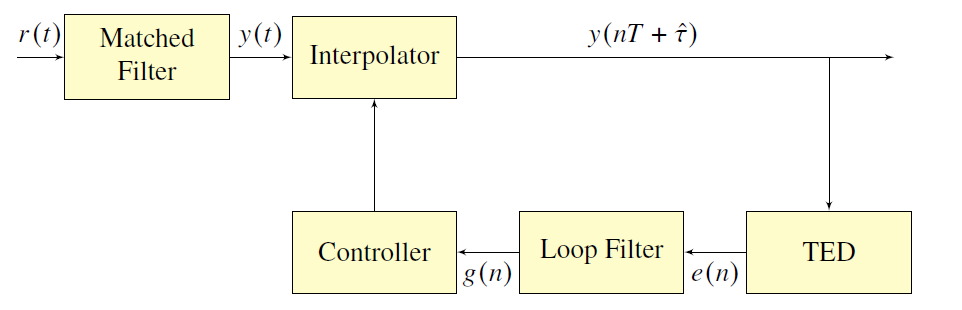
\includegraphics[width=0.7\textwidth]{timing_recovery_block_diagram.png}}}
	\caption{Structure of Timing Recovery PLL}
	\label{fig::timing_recovery_block_diagram_1}
\end{figure}

\noindent In the above figure, the interpolator applies a fractional delay. The timing error detector (TED) measures the time offsets. The loop filter stabilizes error correction, and the interpolator controller manages the interpolation process.

For the timing error detector, three common algorithms are the zero-crossing (ZC) method, the Gardner method, and the M\"{u}ller and Mueller method. For the the experiments, in this lab, we use the zero-crossing method which operates as follows:

\begin{align}
	e(k) = &\text{Re}(x((k-1/2)T_s + \tau))\left[\text{sgn}\{\text{Re}(x((k-1)T_s+\tau))\} - text{sgn}\{\text{Re}(x(kT_s+\tau))\}\right] + \\
	&\text{Im}(x((k-1/2)T_s + \tau))\left[\text{sgn}\{\text{Im}(x((k-1)T_s+\tau))\} - text{sgn}\{\text{Im}(x(kT_s+\tau))\}\right]
\end{align}

\section{Results}
% Results and discussion of the laboratory experiment, including captured outputs, observations, and responses to laboratory questions.

\subsection{Pulse Shaping and Matched Filtering}

Type I Nyquist filters are defined by a rectangular pulse in the frequency domain and a sinc pulse in the time domain. The sinc pulse has zero crossings at $nT$, which produces zero ISI. Because Type I Nyquist filters are a rectangular pulse in the frequency-domain, they have the minimum bandwidth and maximize spectral efficiency. However, there are a couple problems with type I Nyquist filters. First, they are infinite in time. Second, accurate sampling is required. Small timing errors can result in large ISI because the impulse response of a sinc filter decays with $1/t$, which does not converge.

Type II Nyquist filters also have zero crossing at $nT$. However, they have a bandwidth larger than the minimum bandwidth, which allows them to achieve lower ISI sensitivity than type I Nyquist filters. The raised cosine filter is an example of a type II Nyquist filter. Its impulse responses decays with $1/t^3$, which quickly converges in the presence of timing errors.

Next, we compare the frequency response of the SRRC filters for $\beta \in [0,0.1,0.25,0.5,1]$. These frequency responses for these filters are captured in Figures \ref{fig::srrc_freq_response_beta_0} - \ref{fig::srrc_freq_response_beta_1}.

\begin{figure}[H]
	\centerline{\fbox{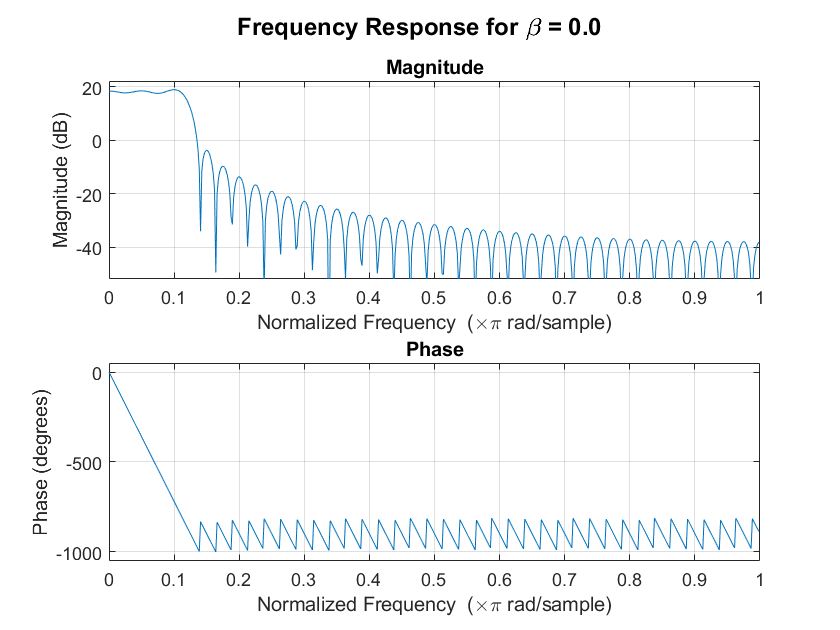
\includegraphics[width=0.5\textwidth]{srrc_freq_response_beta_0.png}}}
	\caption{SRRC Filter Frequency Response with $\beta=0$}
	\label{fig::srrc_freq_response_beta_0}
\end{figure}

\begin{figure}[H]
	\centerline{\fbox{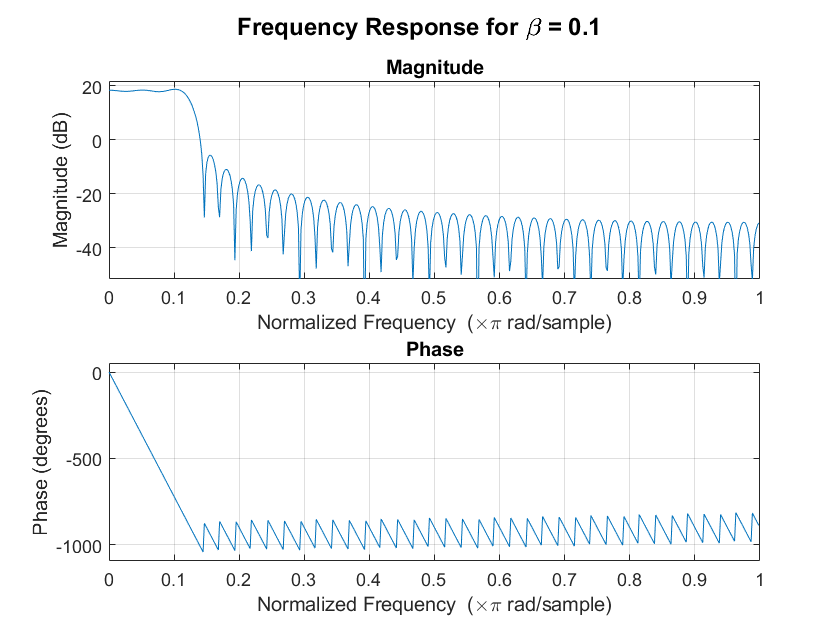
\includegraphics[width=0.5\textwidth]{srrc_freq_response_beta_0_1.png}}}
	\caption{SRRC Filter Frequency Response with $\beta=0.1$}
	\label{fig::srrc_freq_response_beta_0_1}
\end{figure}

\begin{figure}[H]
	\centerline{\fbox{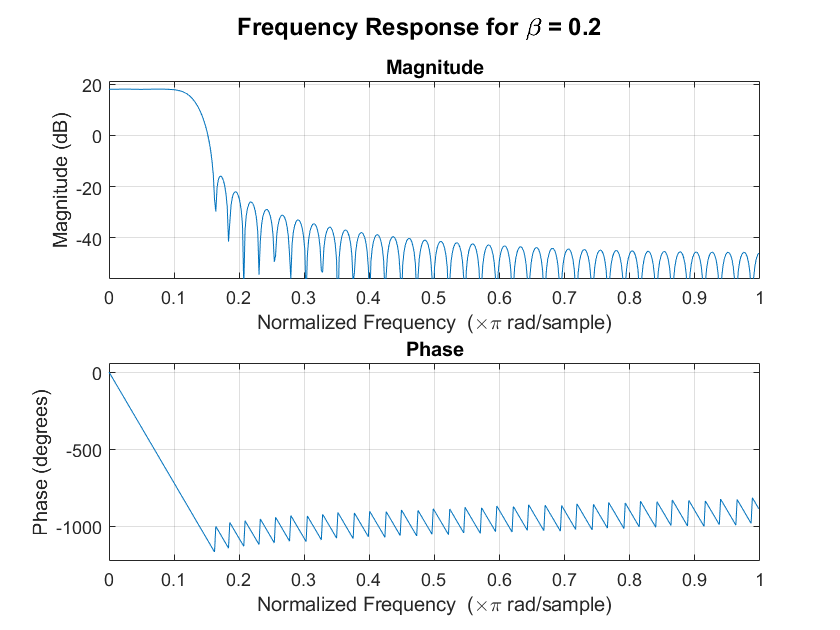
\includegraphics[width=0.5\textwidth]{srrc_freq_response_beta_0_2.png}}}
	\caption{SRRC Filter Frequency Response with $\beta=0.2$}
	\label{fig::srrc_freq_response_beta_0_2}
\end{figure}

\begin{figure}[H]
	\centerline{\fbox{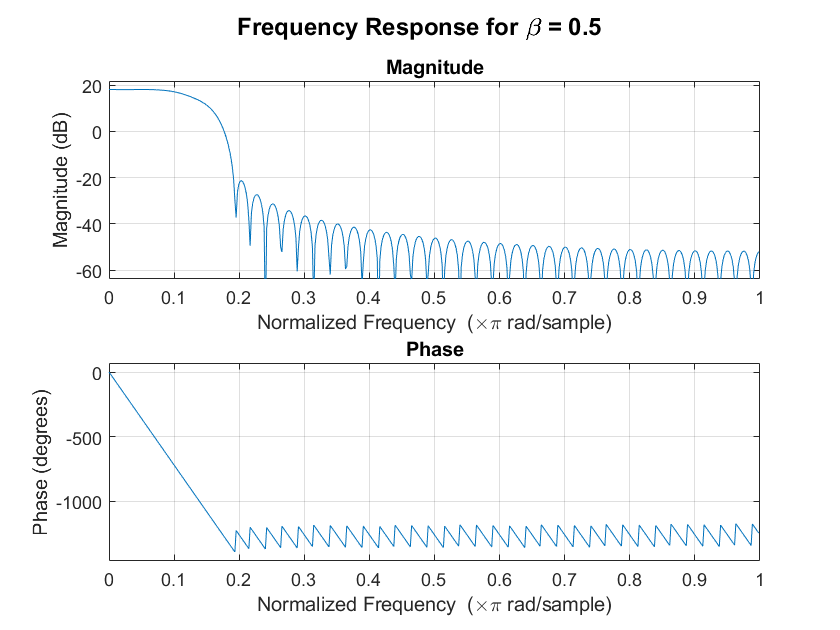
\includegraphics[width=0.5\textwidth]{srrc_freq_response_beta_0_5.png}}}
	\caption{SRRC Filter Frequency Response with $\beta=0.5$}
	\label{fig::srrc_freq_response_beta_0_5}
\end{figure}

\begin{figure}[H]
	\centerline{\fbox{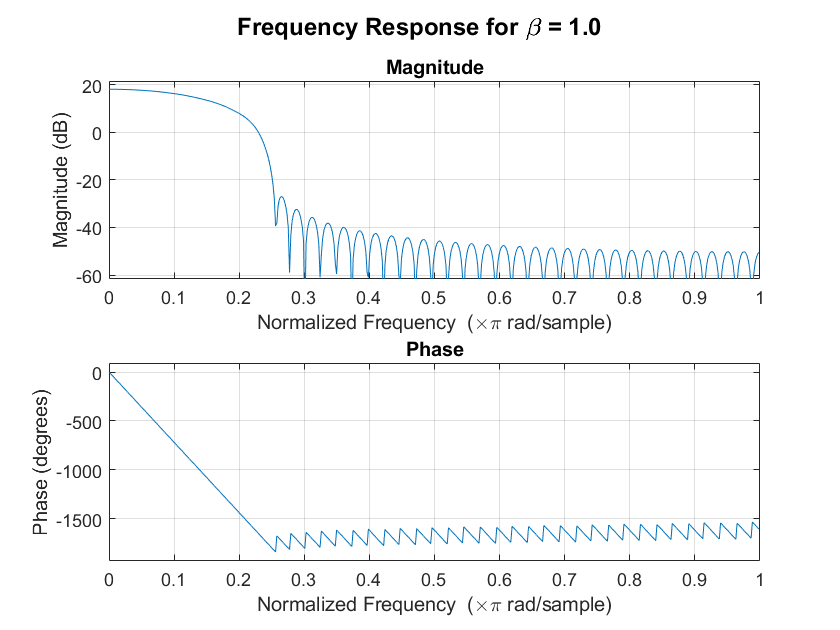
\includegraphics[width=0.5\textwidth]{srrc_freq_response_beta_1.png}}}
	\caption{SRRC Filter Frequency Response with $\beta=1$}
	\label{fig::srrc_freq_response_beta_1}
\end{figure}

\noindent Examining the frequency response of each of the filters, we see that the spectral efficiency is maximized for small values of the rolloff factor, $\beta$. However, the sharp filter transitions required for small $\beta$ increases the complexity of the filter. We can confirm this statement by plotting the impulse response of the filter with $\beta=0$ and $\beta=1$.

\begin{figure}[H]
	\centerline{\fbox{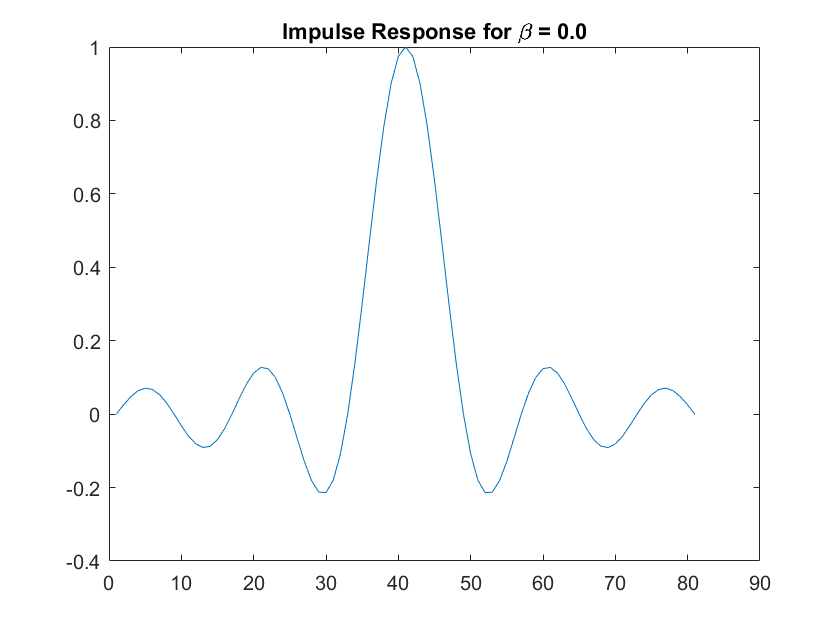
\includegraphics[width=0.5\textwidth]{srrc_impulse_response_beta_0.png}}}
	\caption{SRRC Filter Impulse Response with $\beta=0.0$}
	\label{fig::srrc_impulse_response_beta_0}
\end{figure}

\begin{figure}[H]
	\centerline{\fbox{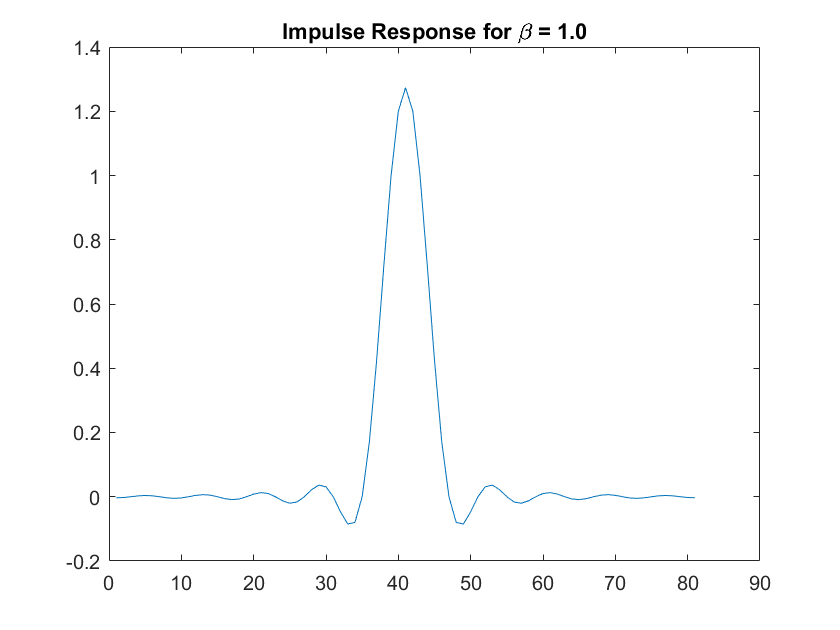
\includegraphics[width=0.5\textwidth]{srrc_impulse_response_beta_1.png}}}
	\caption{SRRC Filter Impulse Response with $\beta=1$}
	\label{fig::srrc_impulse_response_beta_1}
\end{figure}

\noindent Comparing the two impulses responses, we see that the impulse response with $\beta=1$ converges much faster than the impulse response with $\beta=0$. This allows us to truncate the impulse response sooner, which in turn reduces the filter length and complexity.

Finally, we examine how different rolloff factors affect timing recovering performance. To do this we analyze the received filter output for $\beta \in [0.1, 0.5, 0.9]$. Our results are captured in Figures \ref{fig::timing_recovery_beta_0_1} - \ref{fig::timing_recovery_beta_0_9}.

\begin{figure}[H]
	\centerline{\fbox{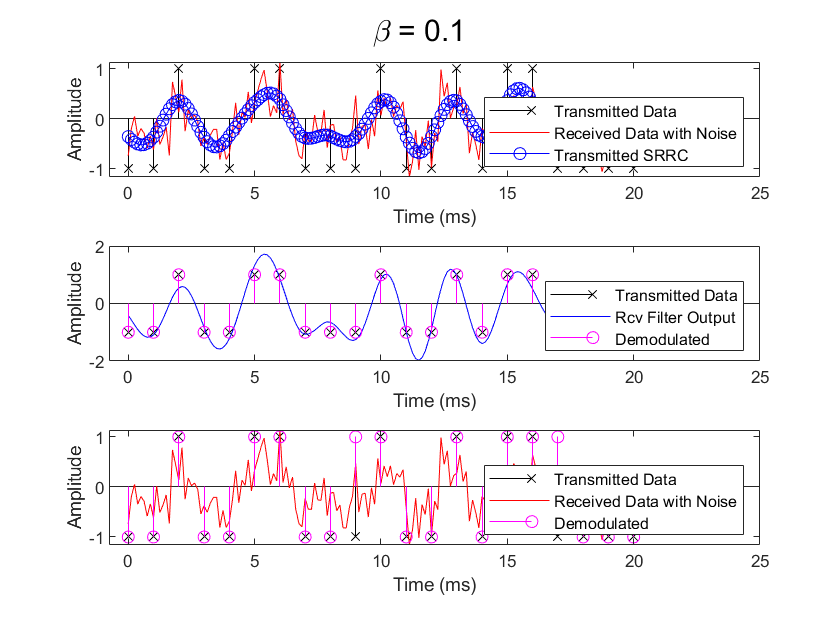
\includegraphics[width=0.5\textwidth]{timing_recovery_beta_0_1.png}}}
	\caption{Timing Recovery with $\beta=0.1$}
	\label{fig::timing_recovery_beta_0_1}
\end{figure}

\begin{figure}[H]
	\centerline{\fbox{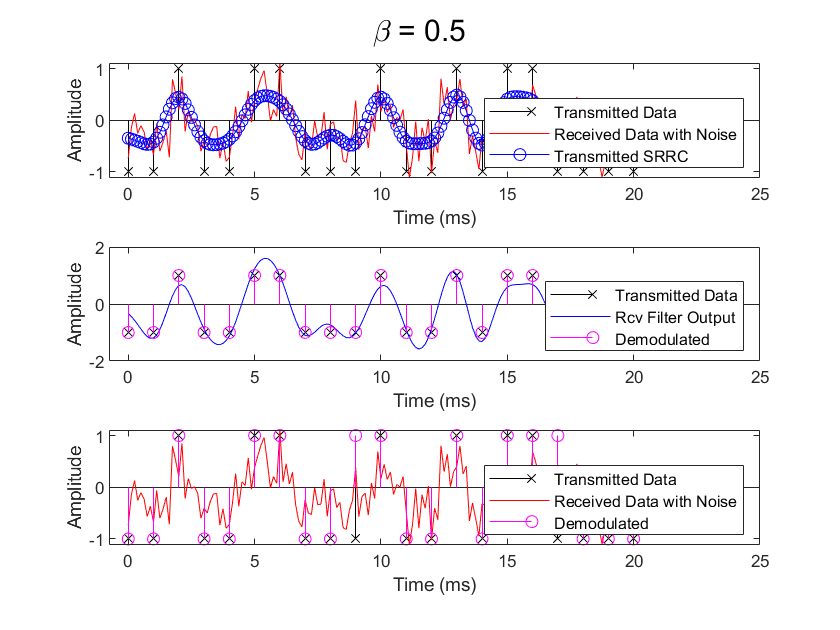
\includegraphics[width=0.5\textwidth]{timing_recovery_beta_0_5.png}}}
	\caption{Timing Recovery with $\beta=0.5$}
	\label{fig::timing_recovery_beta_0_5}
\end{figure}

\begin{figure}[H]
	\centerline{\fbox{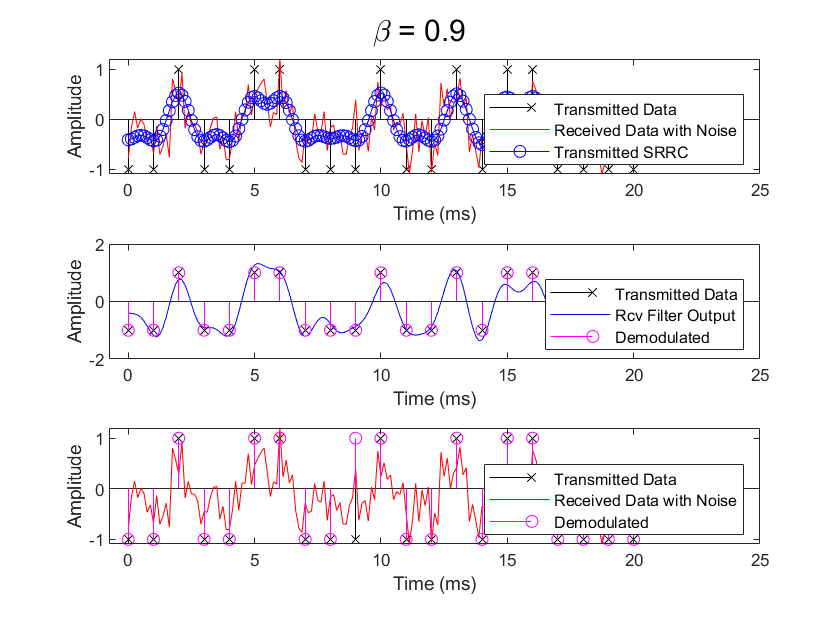
\includegraphics[width=0.5\textwidth]{timing_recovery_beta_0_9.png}}}
	\caption{Timing Recovery with $\beta=0.9$}
	\label{fig::timing_recovery_beta_0_9}
\end{figure}

\noindent The received filter outputs (shown in solid blue) allow us to visualize the effect of various timing offsets. For small values of $\beta$, the receive filter output overshoots the demodulated points more than it does for large values of $\beta$. Given a small timing offset, smaller values of $\beta$ will result in greater timing errors.

\subsection{Timing Error}

In this section, we capture a QPSK constellation with the PlutoSDR. Our captured constellation is shown in Figure \ref{fig::pluto_constellation_raw}.

\begin{figure}[H]
	\centerline{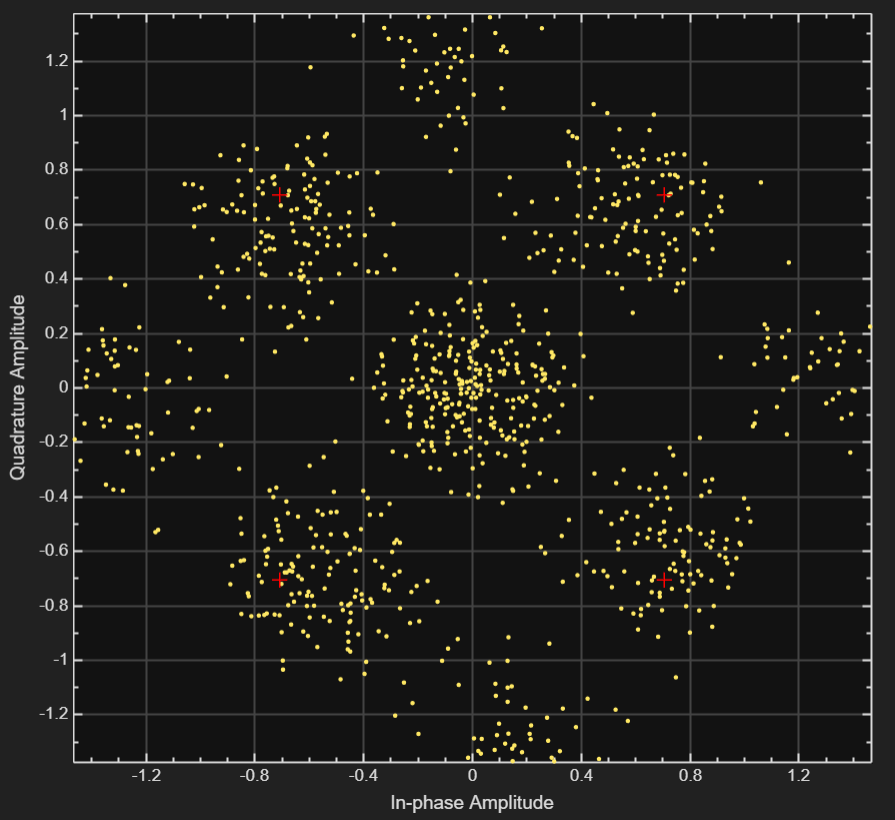
\includegraphics[width=0.5\textwidth]{pluto_constellation_raw.png}}
	\caption{QPSK Constellation Captured with Pluto SDR}
	\label{fig::pluto_constellation_raw}
\end{figure}

\noindent We also leverage code from \texttt{plutoLoopback.m} to sweep timing offsets. If we sweep the timing offsets, we can perform a manual timing compensation. With the best timing compensation, we get the constellation shown in Figure \ref{fig::pluto_constellation_best}.

\begin{figure}[H]
	\centerline{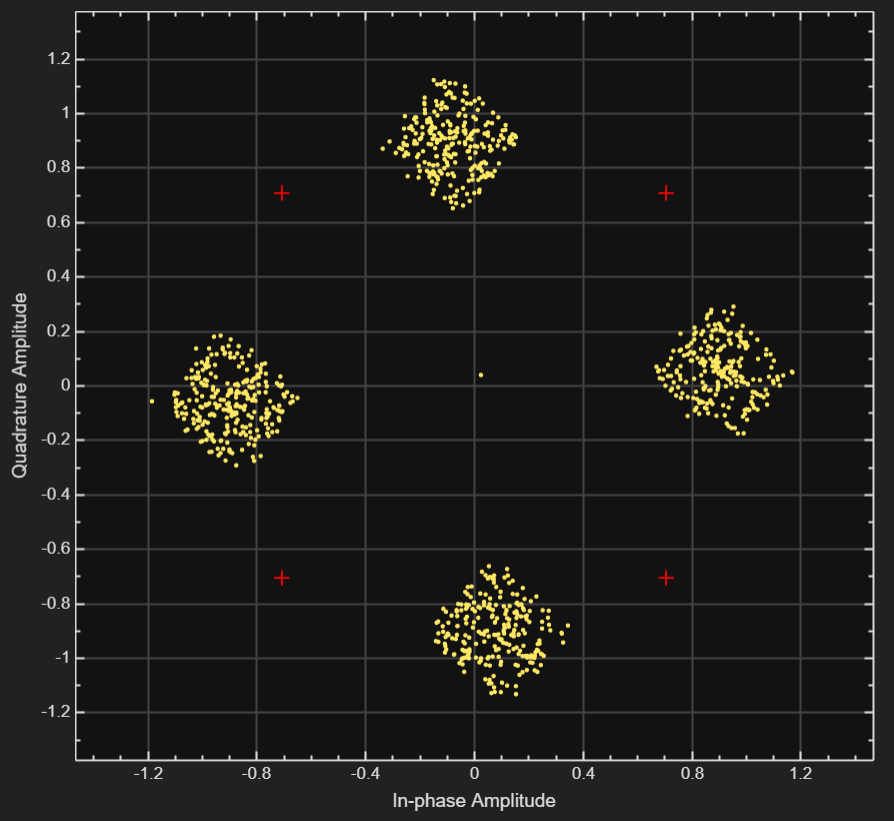
\includegraphics[width=0.5\textwidth]{pluto_constellation_best.png}}
	\caption{QPSK Constellation After Manual Timing Compensation}
	\label{fig::pluto_constellation_best}
\end{figure}

\noindent Before timing compensation, the signal is sampled at non-ideal points, resulting in increased constellation point errors. These increased errors create large clustering patterns in the constellation. After correcting for these timing errors, the errors in the constellation are reduced. However, our constellation remains titled. This titled occurs due to a phase offset in the transmit and receive oscillators. Regardless of what we do with the timing compensation, this phase offset will still be present.

\section{Symbol Timing Compensation}

\subsection{Custom Implementation}

In this section, we perform symbol timing compensation in MATLAB. For this effort, we implement two custom MATLAB implementations and benchmark them against MATLAB's \texttt{comm.SymbolSynchronizer} object. For the first implementation, we connect the textbook-provided routines together following the structure shown in Figure \ref{fig::timing_recovery_block_diagram}. For the second implementation, we replace the textbook-provided routines with custom system objects.

\begin{figure}[H]
	\centerline{\fbox{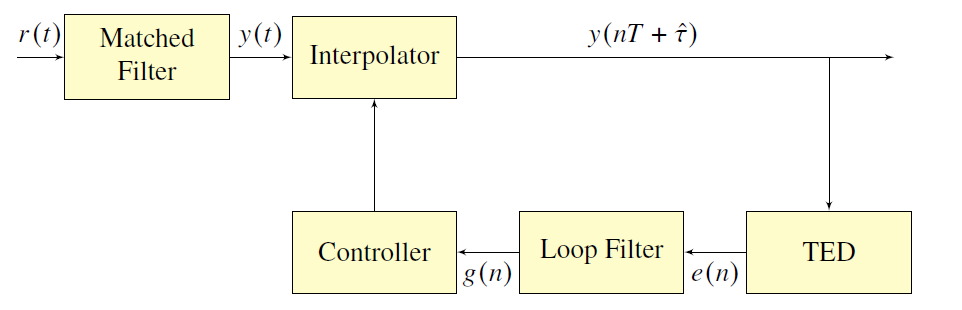
\includegraphics[width=0.7\textwidth]{timing_recovery_block_diagram.png}}}
	\caption{Structure of Timing Recovery PLL}
	\label{fig::timing_recovery_block_diagram}
\end{figure}

\noindent In each implementation, we use a zero-crossing (ZC) timing detector and the following loop filter parameters:

\begin{equation*}
	[N, \zeta, B_{loop}, G_D] = [2, 1, 0.01, 2.7]
\end{equation*}

\noindent To characterize our timing recovery circuits, we create noise-free data with a fixed timing error. We then run the custom implementations and MATLAB's \texttt{comm.SymbolSynchronizer} on the same generated data. In Figure \ref{fig::symbol_sync_no_noise} and \ref{fig::fractional_delay_no_noise}, we plot the synchronized symbols and the fractional delay ($\mu(n)$) output by each routine on the same axes.

\begin{figure}[H]
	\centerline{\fbox{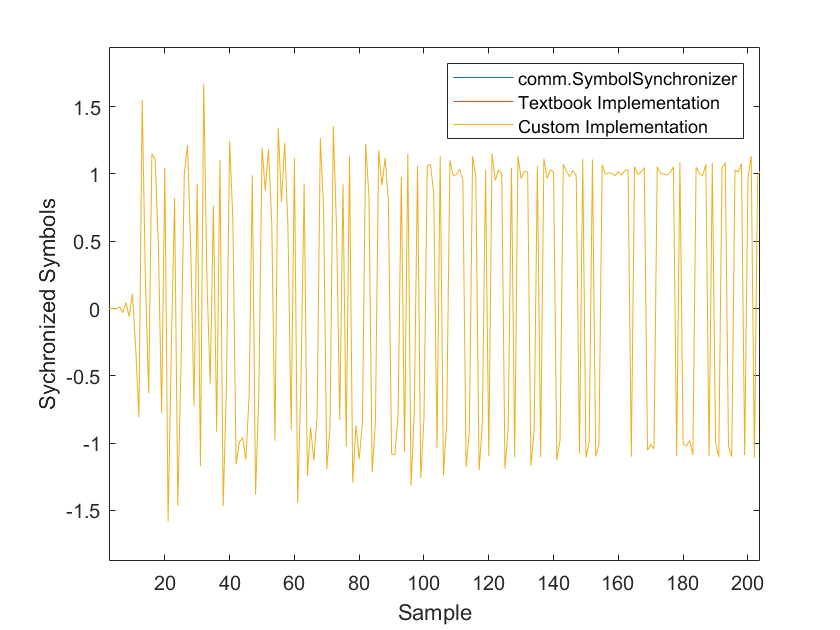
\includegraphics[width=0.5\textwidth]{symbol_sync_no_noise.png}}}
	\caption{Comparison of Synchronized Symbols}
	\label{fig::symbol_sync_no_noise}
\end{figure}

\begin{figure}[H]
	\centerline{\fbox{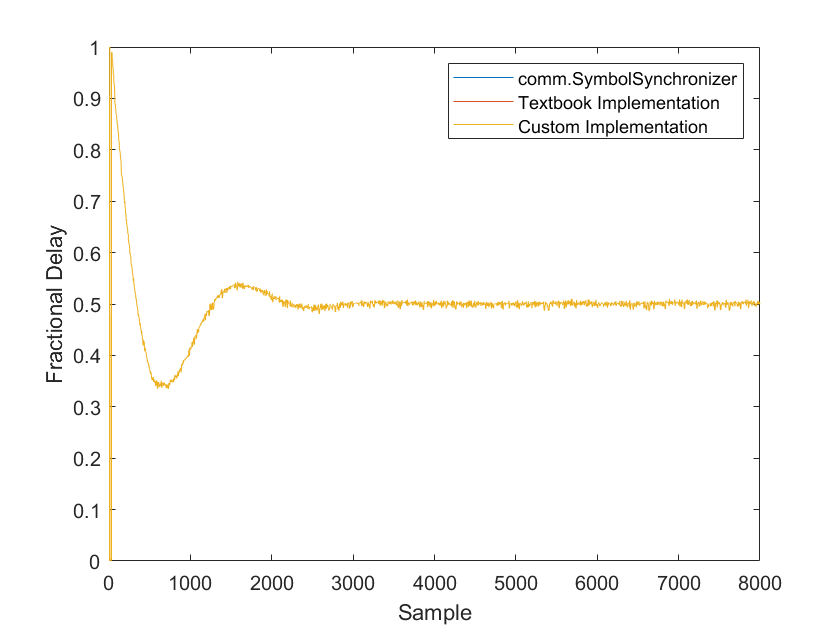
\includegraphics[width=0.5\textwidth]{fractional_delay_no_noise.png}}}
	\caption{Comparison of Fractional Delay}
	\label{fig::fractional_delay_no_noise}
\end{figure}

\noindent Comparing the outputs of each routine, we see that the routine outputs are approximately the same, indicating a correct implementation. We also see that the loop filter parameters cause the fractional delay to converge. For completeness, we also plot the error between the \texttt{comm.SymbolSynchronizer} outputs and the custom routine outputs, which we have included in Figures \ref{fig::symbol_sync_error} and \ref{fig::fractional_delay_error}.

\begin{figure}[H]
	\centerline{\fbox{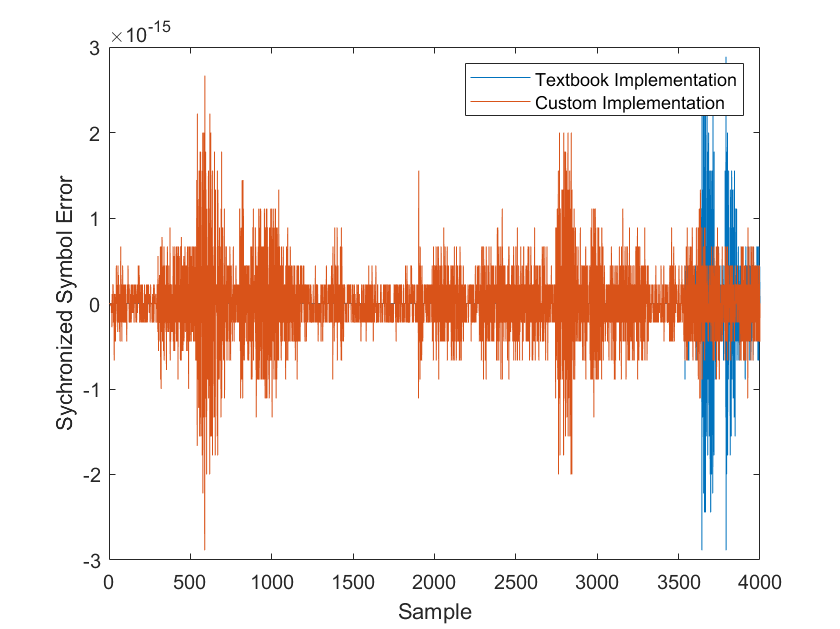
\includegraphics[width=0.5\textwidth]{symbol_sync_error.png}}}
	\caption{Comparison of Synchronized Symbols}
	\label{fig::symbol_sync_error}
\end{figure}

\begin{figure}[H]
	\centerline{\fbox{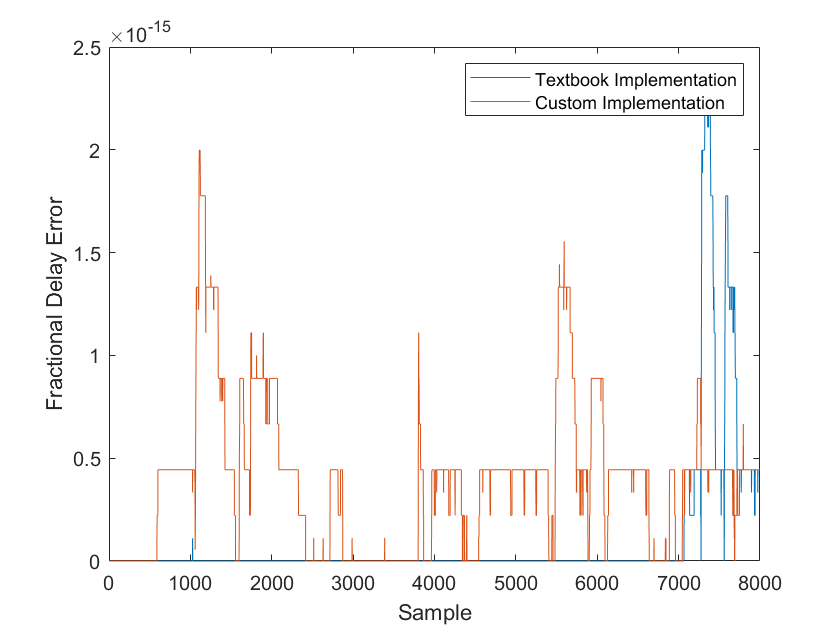
\includegraphics[width=0.5\textwidth]{fractional_delay_error.png}}}
	\caption{Comparison of Fractional Delay}
	\label{fig::fractional_delay_error}
\end{figure}

\noindent With respect to the signal amplitudes, the errors are effectively zero. Therefore, we conclude that our custom implementations are implemented correctly. We also examine the timing offset ($e(n)$) output by the zero-crossing timing error detector. This value is not output by the \texttt{comm.SymbolSynchronizer}. However, we can examine this timing offset for each of our implementations. These timing offsets are included in Figure \ref{fig::timing_offset}. 

\begin{figure}[H]
	\centerline{\fbox{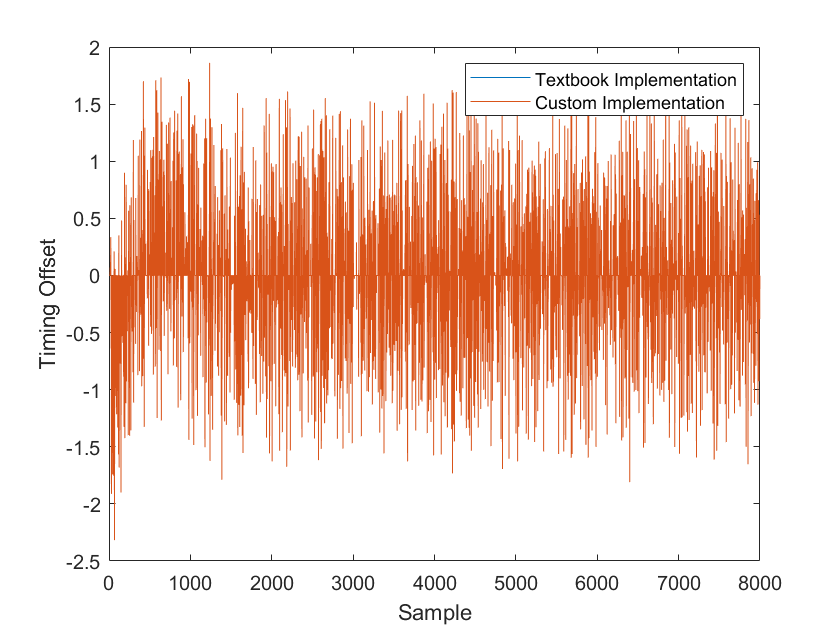
\includegraphics[width=0.5\textwidth]{timing_offset.png}}}
	\caption{Timing Offset Output by ZC TED}
	\label{fig::timing_offset}
\end{figure}

\noindent Examining the timing offsets, we see that the both routines output the same values. We can also draw a few other conclusions. First, we see that the timing offset alternates between zero and non-zero values. This is expected because the timing error detector only outputs non-zero values when it receives a trigger, which happens roughly every other cycle. Additionally, we see that the timing offset rapidly oscillates even after the fractional delay has converged. However, we have previously shown that this is not an error because the fractional delay converges and because the results are consistent with the \texttt{comm.SymbolSynchronizer} object.

A better indication of the PLL performance is the fractional delay error (i.e. the difference between the measured fractional delay and configured fractional delay). Figure \ref{fig::delay_error_no_noise} display this error for a noise-free signal, and Figures \ref{fig::delay_error_20dB_snr} and \ref{fig::delay_error_10dB_snr} display this error for 20dB and 10dB SNR respectively. 

\begin{figure}[H]
	\centerline{\fbox{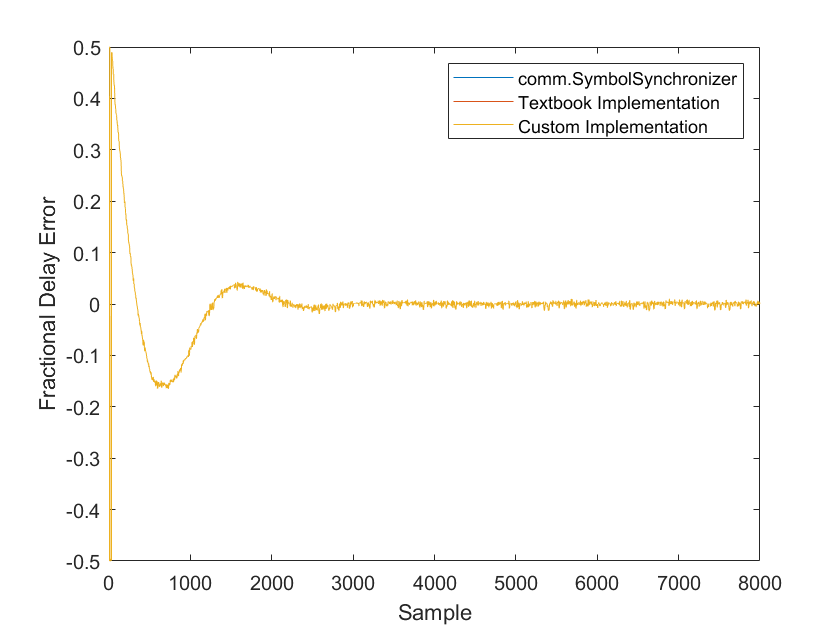
\includegraphics[width=0.5\textwidth]{delay_error_no_noise.png}}}
	\caption{Fractional Delay Error for Noise Free Signal}
	\label{fig::delay_error_no_noise}
\end{figure}

\begin{figure}[H]
	\centerline{\fbox{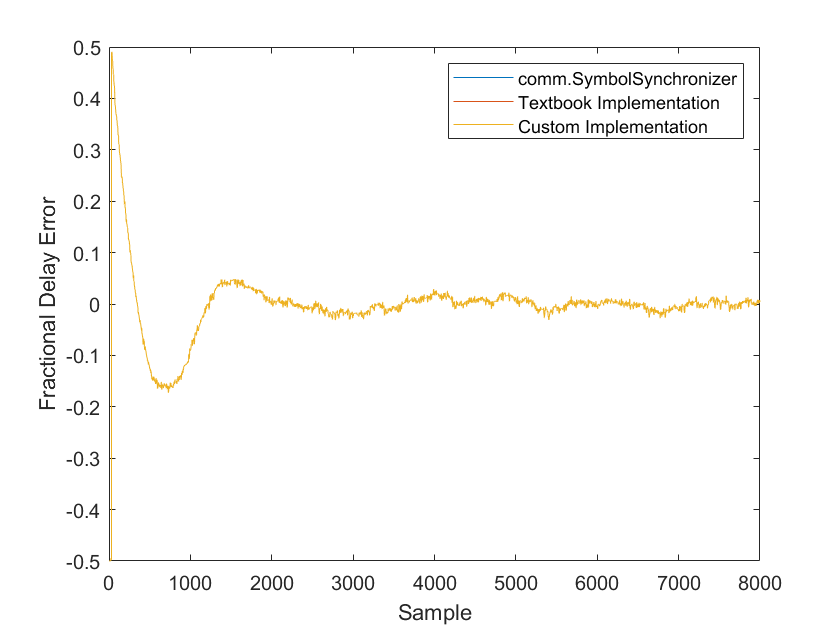
\includegraphics[width=0.5\textwidth]{delay_error_20dB_snr.png}}}
	\caption{Fractional Delay Error for Signal with 20dB SNR}
	\label{fig::delay_error_20dB_snr}
\end{figure}

\begin{figure}[H]
	\centerline{\fbox{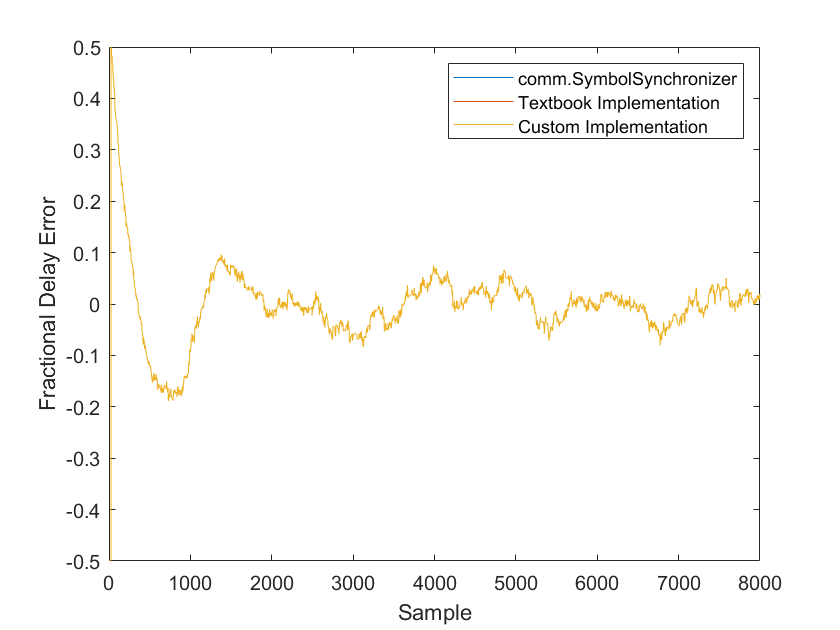
\includegraphics[width=0.5\textwidth]{delay_error_10dB_snr.png}}}
	\caption{Fractional Delay Error for Signal with 10dB SNR}
	\label{fig::delay_error_10dB_snr}
\end{figure}

\noindent Comparing each of the figures, we see that the timing compensation is dependent on the SNR of the received signal (better SNR leads to better timing compensation). Additionally, the custom routines produce identical results to the MATLAB \texttt{comm.SymbolSynchronizer} object across different values of SNR.

\subsection{Performance}

Next, we analyze the performance of the timing compensation logic when we apply a slowly-changing timing offset. For this experiment, we specifically allow the timing offset to drift by a hundredth of symbol every 1024 symbols. In Figure \ref{fig::fractional_delay_timing_offset}, we show the measured fractional delay with a 20 dB SNR, and in Figure \ref{fig::fractional_delay_error_timing_offset}, we show the fractional delay error.

\begin{figure}[H]
	\centerline{\fbox{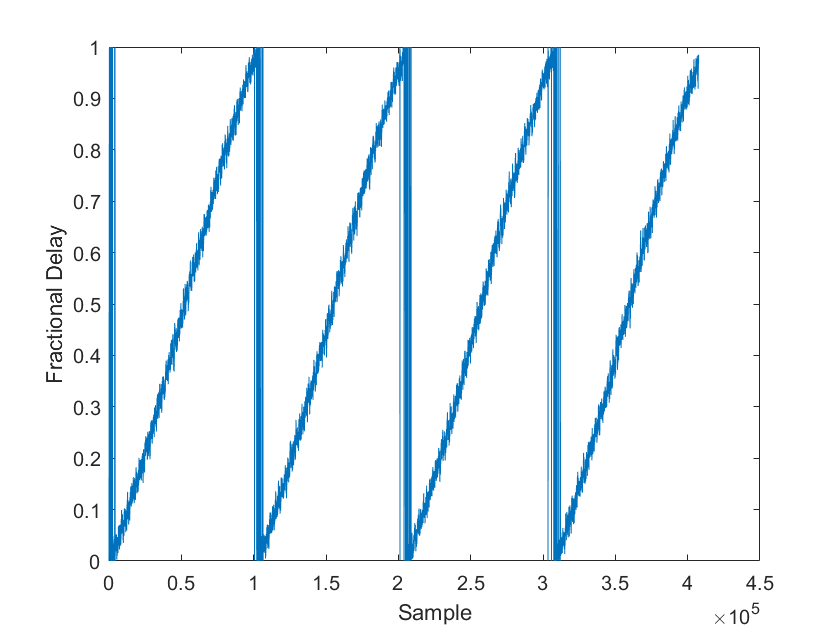
\includegraphics[width=0.5\textwidth]{fractional_delay_timing_offset.png}}}
	\caption{Fractional Delay Measured for Data with Slowly Varying Timing Delay}
	\label{fig::fractional_delay_timing_offset}
\end{figure}

\begin{figure}[H]
	\centerline{\fbox{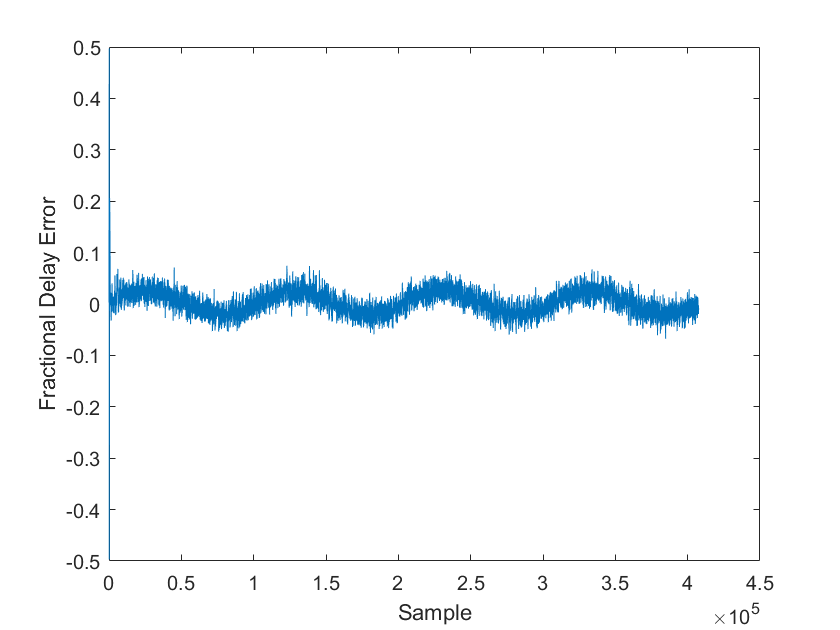
\includegraphics[width=0.5\textwidth]{fractional_delay_error_timing_offset.png}}}
	\caption{Fractional Delay Error Measured for Data with Slowly Varying Timing Delay}
	\label{fig::fractional_delay_error_timing_offset}
\end{figure}

\noindent Examining the figure outputs, we see that the fractional delay increases linearly with time as expected. Additionally, we see that the timing error converges to zero. However, compared to the outputs shown in Figures \ref{fig::delay_error_no_noise}, the fractional delay error oscillates at steady state. In Figure \ref{fig::constellations_with_timing_correction}, we show the constellations before and after timing compensation. For this analysis, we use BPSK modulation.
 
\begin{figure}[H]
	\centerline{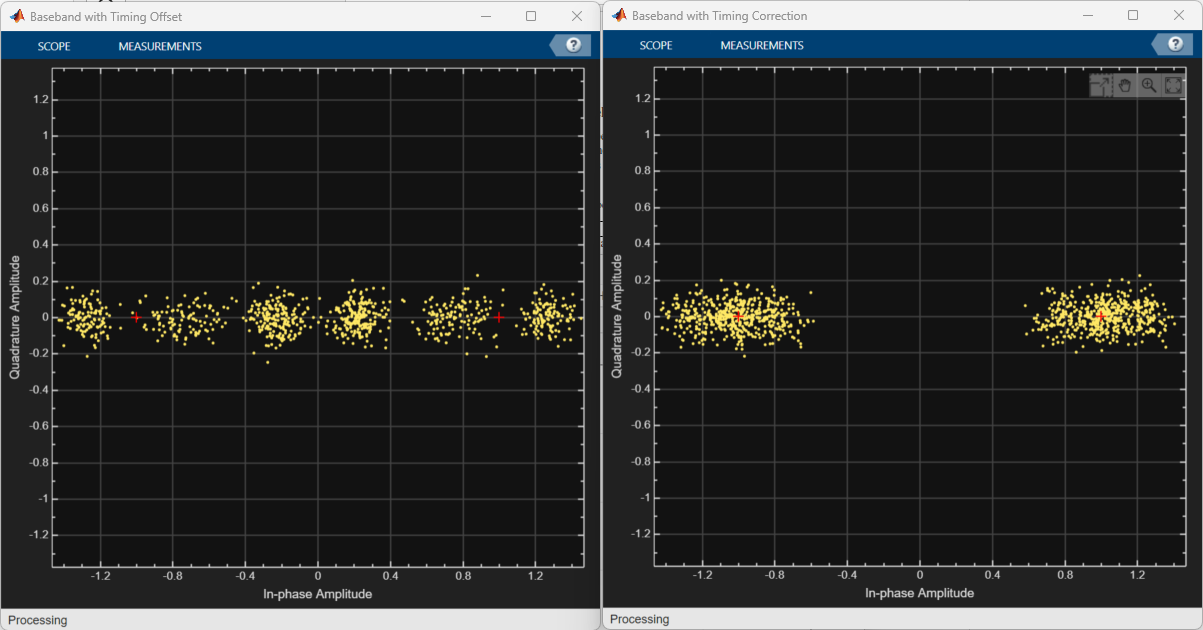
\includegraphics[width=0.8\textwidth]{constellations_with_timing_correction.png}}
	\caption{Constellations Before Timing Compensation (Left) and After Timing Compensation (Right)}
	\label{fig::constellations_with_timing_correction}
\end{figure}

\noindent Before timing compensation, the constellation does not match closely with our expectations for BPSK modulation. However, after timing compensation, all the received data is clustered around $\pm 1$ as expected.

Next, we plot the error vector magnitude (EVM) against SNR and include the results in Figure \ref{fig::evm_vs_snr}. Examining the plot, we see that the error magnitude vector fall linearly with SNR for low values of SNR before converging to a final value.
\begin{figure}[H]
	\centerline{\fbox{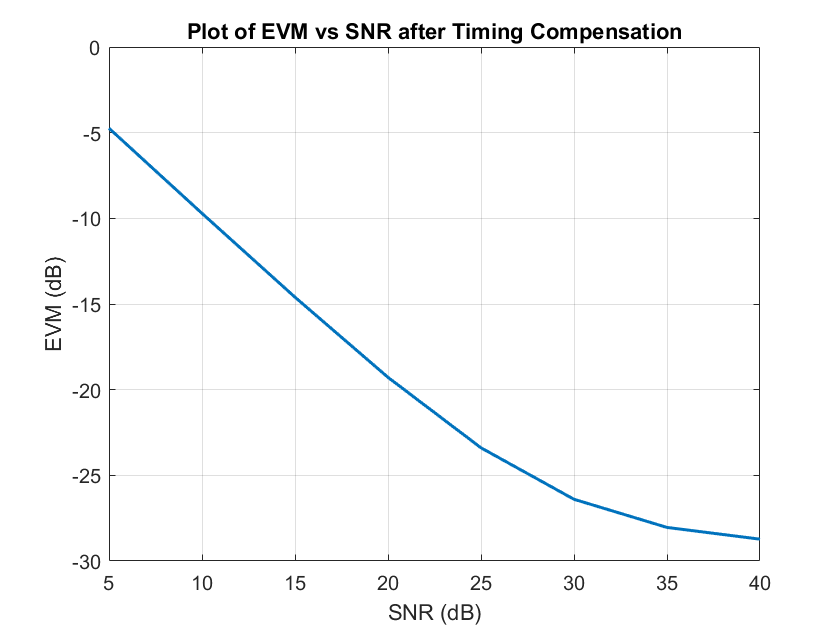
\includegraphics[width=0.5\textwidth]{evm_vs_snr.png}}}
	\caption{Plot of EVM vs SNR}
	\label{fig::evm_vs_snr}
\end{figure}

\noindent We can perform similar analysis with a phase offset instead of a timing offset. For this analysis, we use a phase error of $\pi/8$ radians. Our results are illustrated in Figure \ref{fig::evm_vs_snr_with_phase_offset}.

\begin{figure}[H]
	\centerline{\fbox{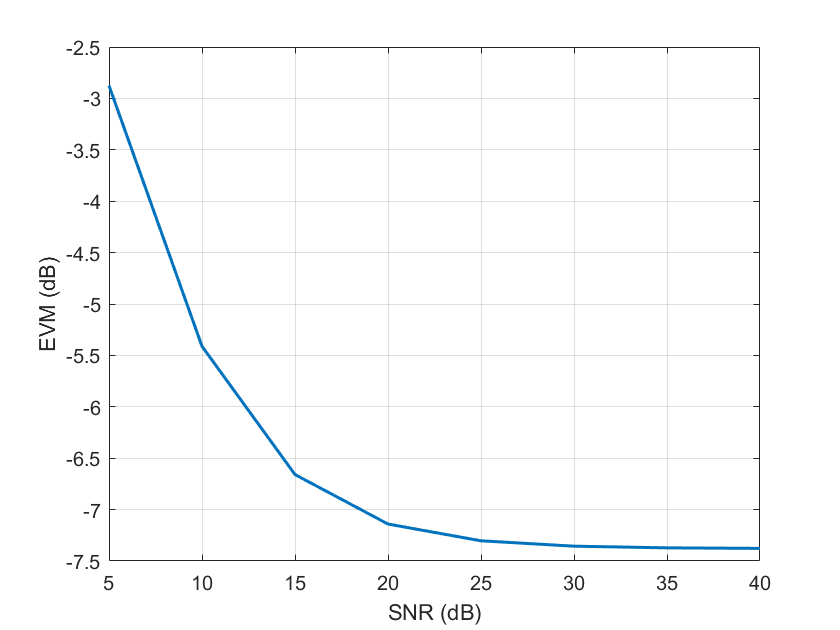
\includegraphics[width=0.5\textwidth]{evm_vs_snr_with_phase_offset.png}}}
	\caption{Plot of EVM vs SNR for $\protect\pi/8$ Phase Offset}
	\label{fig::evm_vs_snr_with_phase_offset}
\end{figure}

\noindent Compared to Figure \ref{fig::evm_vs_snr}, the EVM is almost 10 dB worse in steady state. This occurs because the phase error has become the limiting factor for the EVM measurement. With an added phase offset of $\pi/8$, we again display the constellation before and after modulation.

\begin{figure}[H]
	\centerline{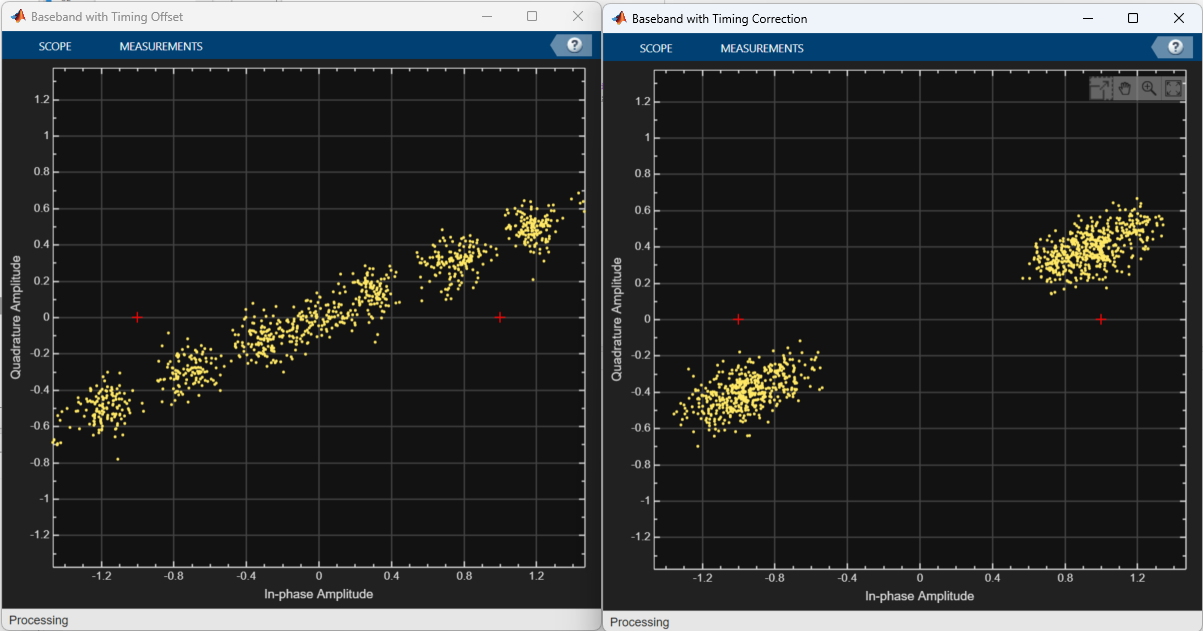
\includegraphics[width=0.8\textwidth]{constellations_with_timing_correction_phase_offset.png}}
	\caption{Constellations with Phase Offset Before and After Timing Compensation}
	\label{fig::constellations_with_timing_correction_phase_offset}
\end{figure}

\noindent Examining Figure \ref{fig::constellations_with_timing_correction_phase_offset}, we see that the timing compensation correctly clusters each of the received symbols. However, the symbols have been rotated due to phase error. To account for the phase error, we can use differential modulation (DBPSK vs BPSK). For our DBPSK demodulation, we use the phase difference between adjacent samples to determine the transmitted symbols. We leverage the following equation to find the phase different between samples:

\begin{equation}
	y[n] = A[n]e^{j\phi[n]}*e^{-j\phi[n-1]}
\end{equation}

\noindent Then, we compute the resulting EVM, which is plotted against SNR in Figure \ref{fig::evm_vs_snr_dbpsk}.

\begin{figure}[H]
	\centerline{\fbox{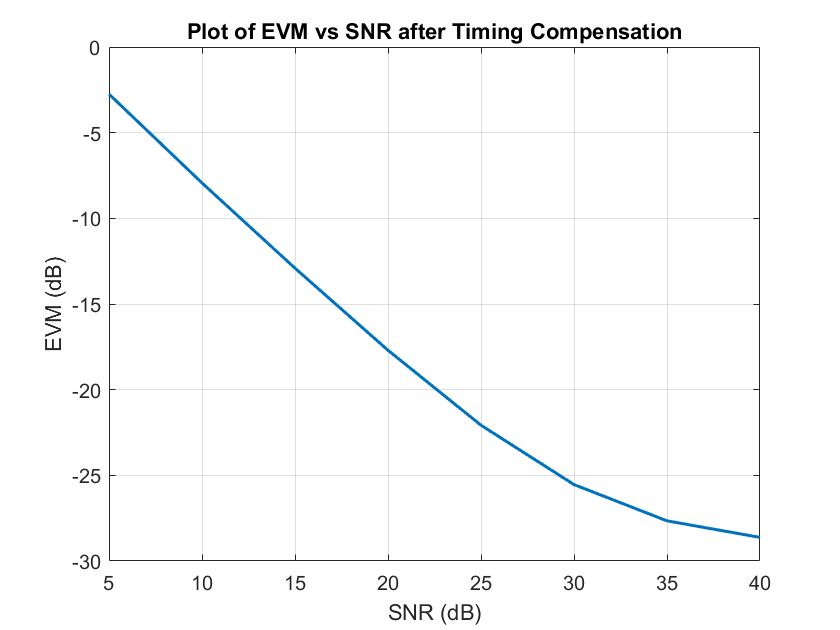
\includegraphics[width=0.5\textwidth]{evm_vs_snr_dbpsk.png}}}
	\caption{EVM vs SNR for DBPSK Modulation with a $\protect\pi/8$ Phase Offset}
	\label{fig::evm_vs_snr_dbpsk}
\end{figure}

Compared to Figure \ref{fig::constellations_with_timing_correction_phase_offset}, we see that the EVM has substantially improved. However, it does deviate slightly from our EVM plots when we use BPSK with no phase offset. This occurs because noisy samples are used to find phase differences.

\section{Adding Pieces Together}

In this section, we review the timing recovery circuit and the sample rates of each of its blocks. A block diagram of the timing recovery circuit is included in Figure \ref{fig::timing_recovery_block_diagram_2}. Our timing recovery circuit (with the exception of the "asynchronous FIFO" interface) runs at a sample rate of $2/T_s$, where $T_s$ is the symbol duration. As a result, our receive filter must output samples at twice the symbol rate.

	The interpolator receives a fractional delay, which is updated each trigger. It outputs outputs the signal with fractional delay and delayed-version of the trigger to an "asynchronous FIFO" interface. This FIFO stores the filter output every time it receives a trigger and outputs 1 sample per symbol. Triggers occur on average once per cycle as well, so there is little risk of overflow. To the design is resilient, we may clear the FIFO if it starts to overflow. However, this feature is not included in our implementation.
	
	The timing error detector implements the zero-crossing algorithm. As such, it requires an additional interpolator, which is not shown. The timing error detector outputs an error every time it receives a trigger. When it does not receive a trigger, the timing error detector outputs a zero. The loop filter uses a PI controller and controls the interpolation controller, which, in turn, creates triggers and updates the fractional delay parameter on each trigger.
	
\begin{figure}[H]
	\centerline{\fbox{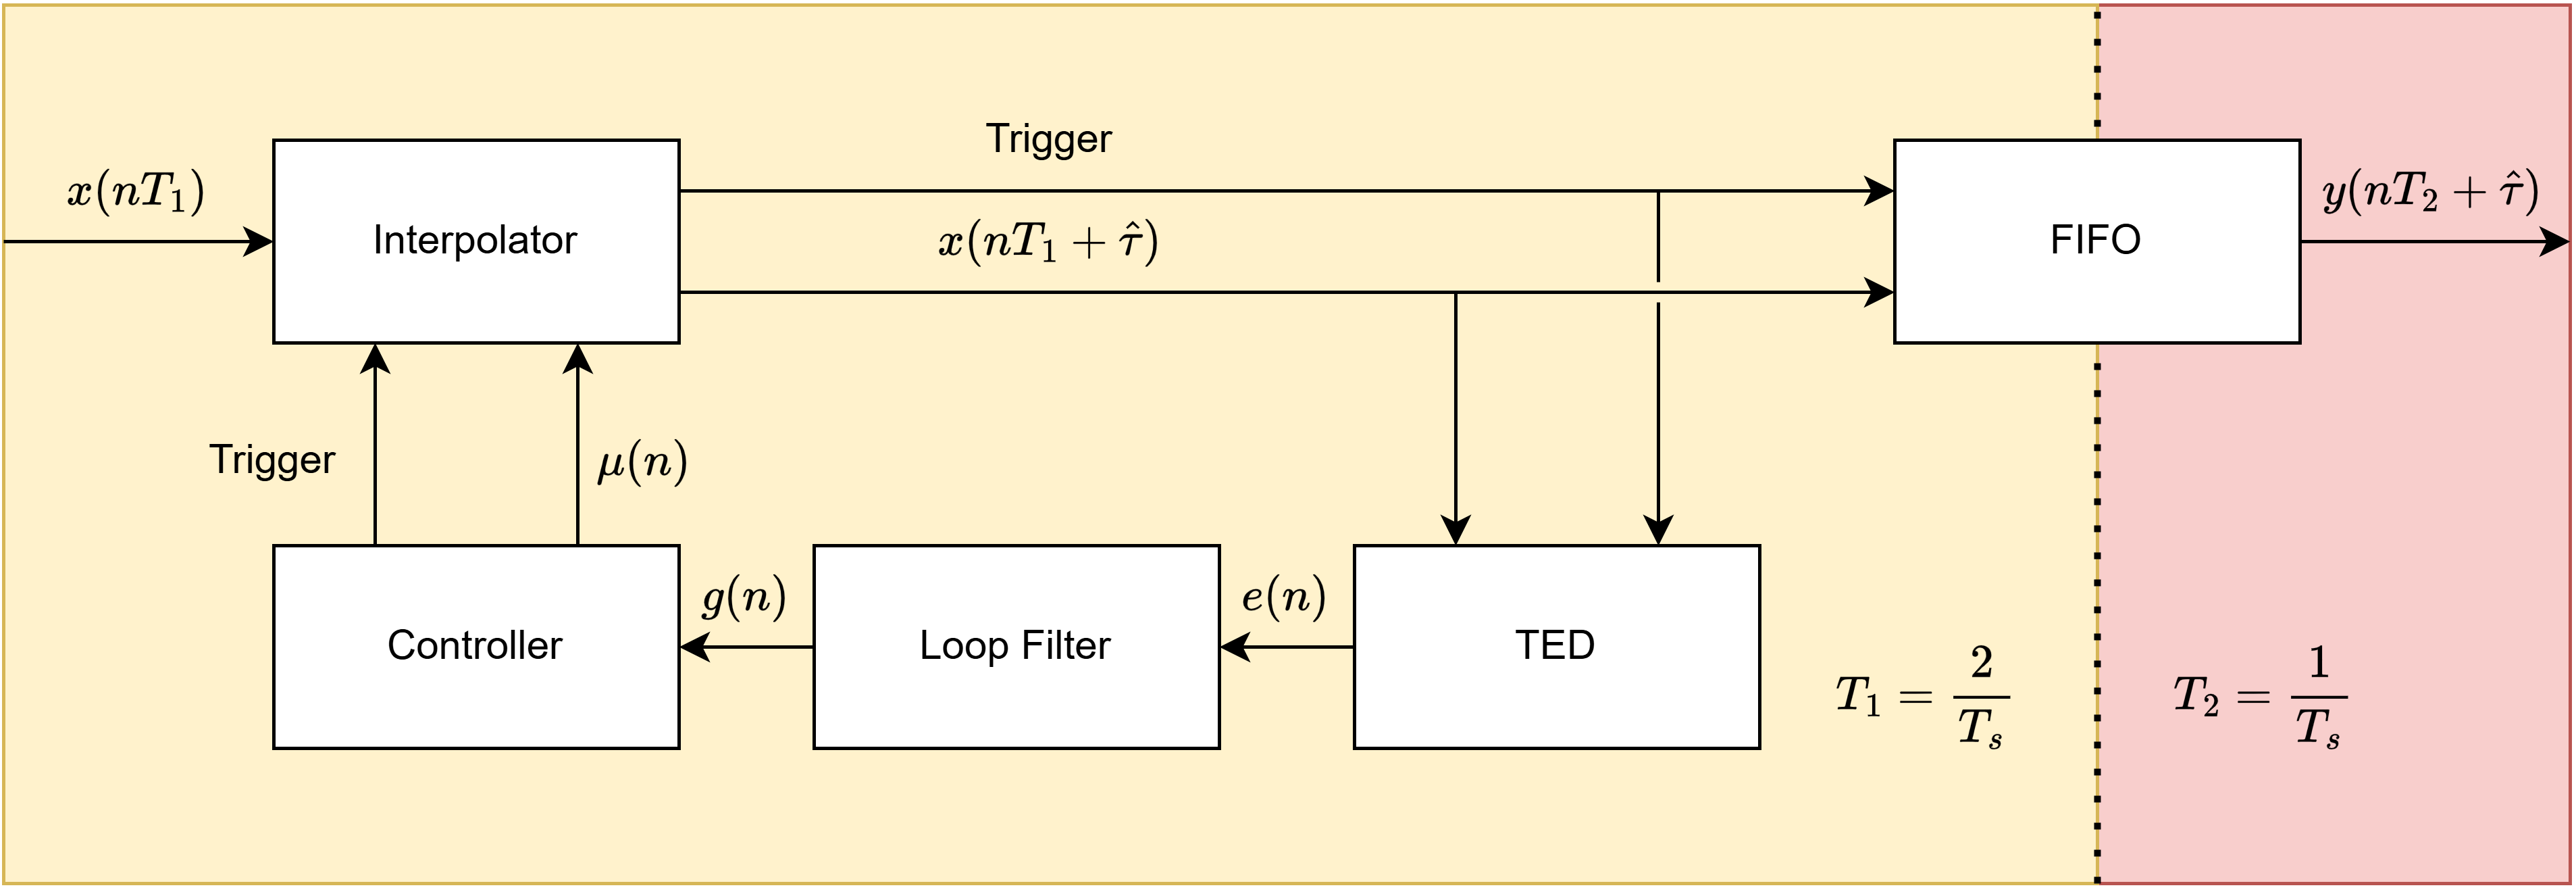
\includegraphics[width=0.7\textwidth]{timing_recovery_block_diagram_2.png}}}
	\caption{Block Diagram of Timing Recovery Circuit}
	\label{fig::timing_recovery_block_diagram_2}
\end{figure}

We evaluate the performance of the timing recovery block by measuring the EVM under a couple different conditions. First we measure the EVM with no timing offsets (i.e. the ideal base case). These results are included in Figure \ref{fig::evm_no_timing_offset}.

\begin{figure}[H]
	\centerline{\fbox{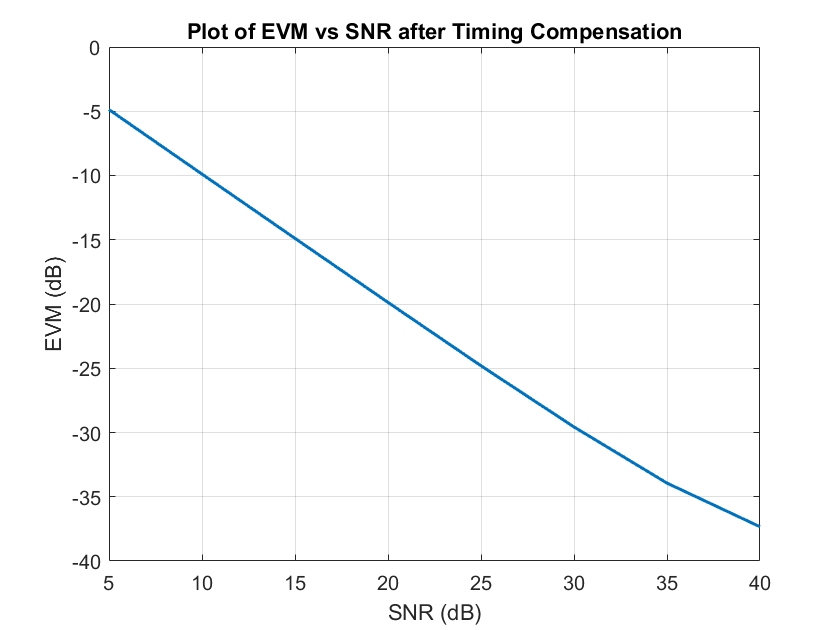
\includegraphics[width=0.5\textwidth]{evm_no_timing_offset.png}}}
	\caption{EVM with No Timing Offsets}
	\label{fig::evm_no_timing_offset}
\end{figure}

Examining the figure output, we see that the EVM is roughly the same as the input SNR. This is the expected result because the EVM is the ratio of the error power to the reference constellation power. The reference constellation power is the signal power and the error power is the power of the additive noise. Therefore EVM and input SNR are the same for this case. Next, we consider the EVM when we apply a fixed timing offset of $0.25T_s$. These results are included in Figure \ref{fig::evm_0p25_symbol_offset}.

\begin{figure}[H]
	\centerline{\fbox{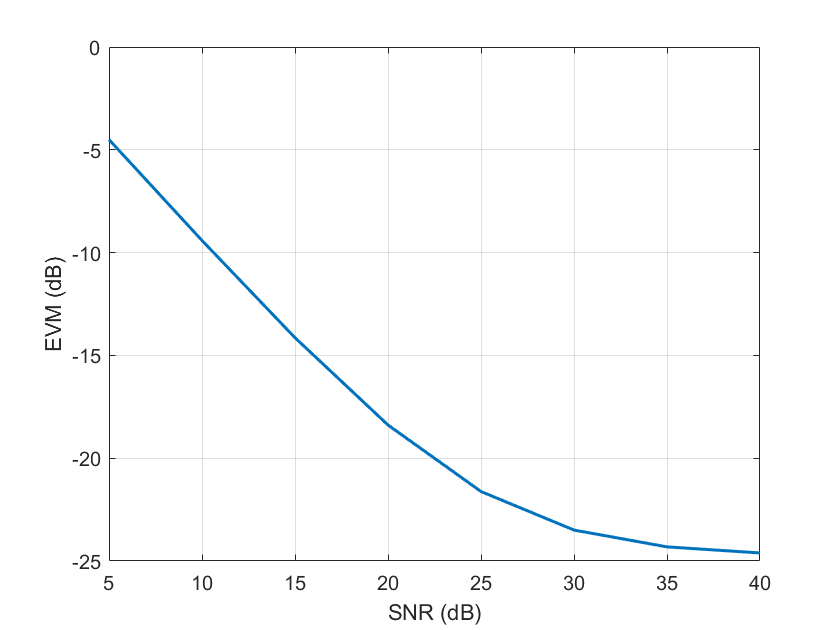
\includegraphics[width=0.5\textwidth]{evm_0p25_symbol_offset.png}}}
	\caption{EVM with $\protect{0.25T_s}$ Symbol Offset}
	\label{fig::evm_0p25_symbol_offset}
\end{figure}

Examining the figure, we see that the EVM is approximately the same as the SNR for low SNR but converges to a constant value as the SNR gets large. At these high SNR points, the timing recovery circuit is the limiting factor for the EVM. Next, we examine the performance when we apply a phase offset of $\pi/8$ instead of a timing error. These results are included in \ref{fig::evm_pi_8_phase_offset}.

\begin{figure}[H]
	\centerline{\fbox{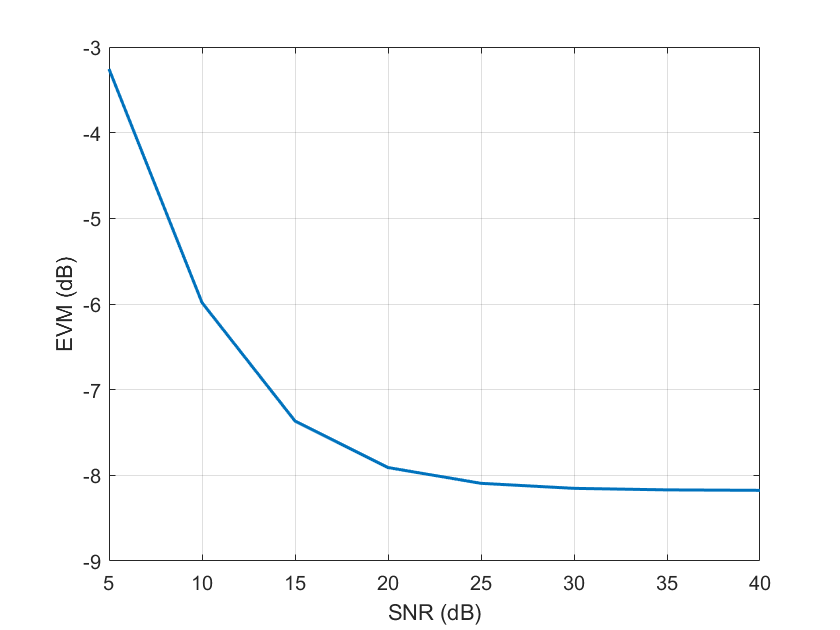
\includegraphics[width=0.5\textwidth]{evm_pi_8_phase_offset.png}}}
	\caption{EVM with $\protect\pi/8$ Phase Offset}
	\label{fig::evm_pi_8_phase_offset}
\end{figure}

Comparing the results of Figure \ref{fig::evm_pi_8_phase_offset} to Figures \ref{fig::evm_no_timing_offset} and \ref{fig::evm_0p25_symbol_offset}, we see that the EVM is degraded substantially. We can make sense of this value by computing the error between a unit-power constellation point and a constellation point without noise and a phase error of $\pi/8$. Doing so, we find:

\begin{equation}
	\text{error} = (1 - \cos\pi/8)^2 + \sin^2\pi/8 = 1 - 2\cos\pi/8 + \cos^2\pi/8 + \sin^2\pi/8 = 2 - 2\cos\pi/8 \approx 0.15224 
\end{equation}

\noindent which corresponds to an EVM of 

\begin{equation}
	\text{EVM}_{\text{dB}} = 10\log_{10}\left(\text{error}\right) \approx 10\log_{10}(0.15224) \approx -8.17\ \text{dB}
\end{equation}

\noindent Note that this value is consistent with our high-SNR EVM measurement. We can visualize the timing error detector performance in the presence of phase error by examining the constellation, which is shown in Figure \ref{fig::evm_pi_8_phase_offset}.

\begin{figure}[H]
	\centerline{\fbox{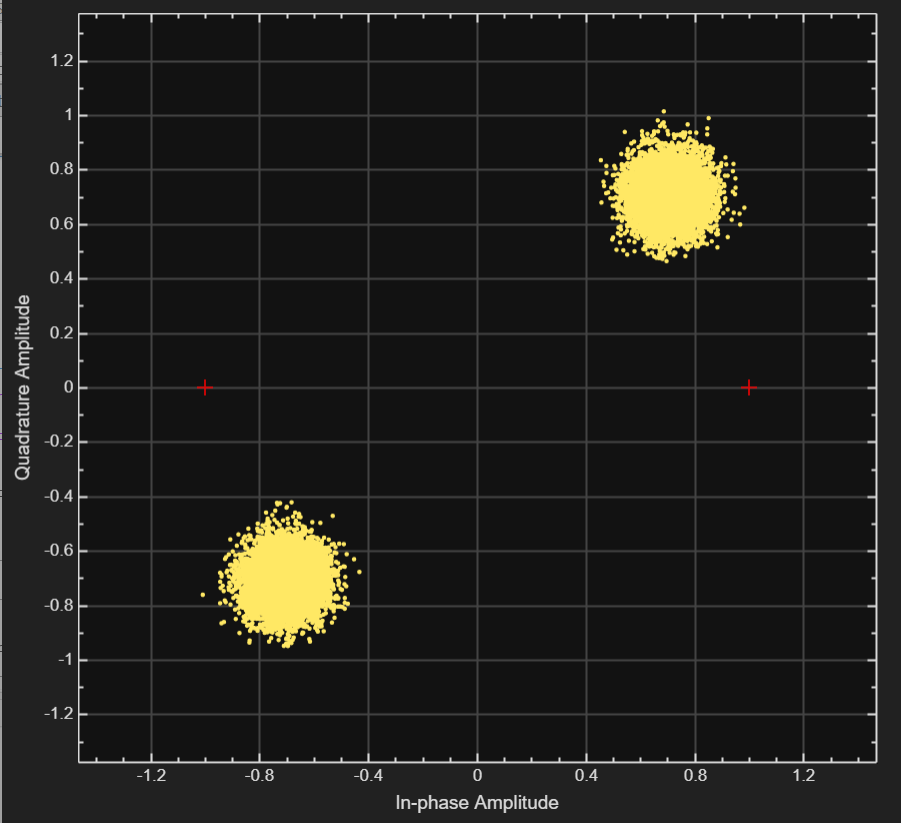
\includegraphics[width=0.5\textwidth]{constellation_phase_error.png}}}
	\caption{Constellation after Timing Compensation with 20 dB SNR and a $\protect\pi/8$ Phase Offset}
	\label{fig::constellation_phase_error}
\end{figure}

\noindent Examining the Figure we see that the phase error creates a rotation in the complex plane, which artificially distorts our EVM metric. One way to handle this phase error is to use differential modulation. We specifically can use DBPSK modulation instead of BPSK modulation. Then, we compute the resulting constellation points as follows:

\begin{equation}
	y[n] = A[n]e^{j\phi[n]}*e^{-j\phi[n-1]}
\end{equation}

\noindent The results of this experiment are shown in Figure \ref{fig::evm_dpsk_modulation}.

\begin{figure}[H]
	\centerline{\fbox{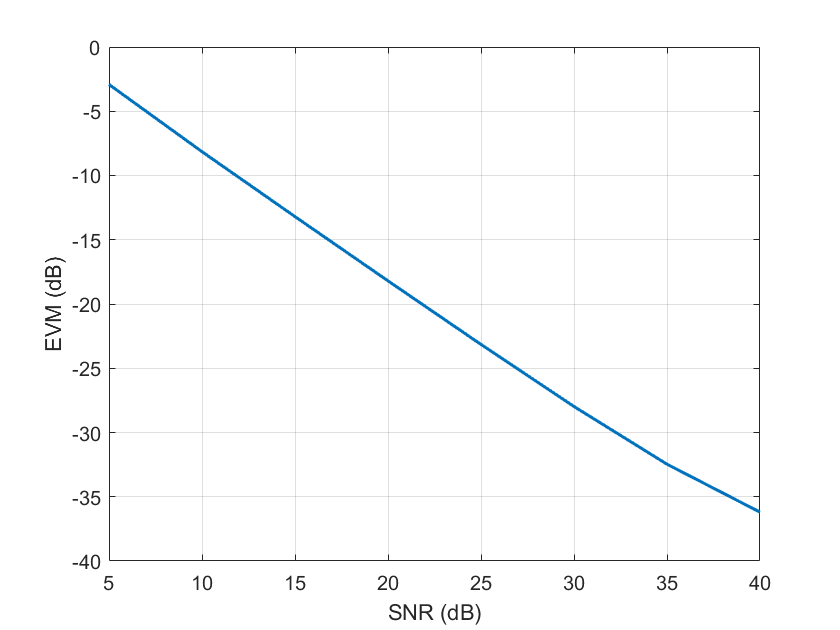
\includegraphics[width=0.5\textwidth]{evm_dpsk_modulation.png}}}
	\caption{EVM with $\protect\pi/8$ Phase Offset After Differential Demodulation}
	\label{fig::evm_dpsk_modulation}
\end{figure}

\noindent Examining the Figure output, we note that it is close to the result shown in Figure \ref{fig::evm_no_timing_offset}. However, the EVMs are slightly worse because our phase offset is computed based from a noisy input, which leads to more noise in the output.

\section{Testing on Hardware}

In this section, we perform timing compensation with the PlutoSDR. We start by transmitting a DBPSK reference signal, so we do not have to worry about the phase offset that we observed in Figure \ref{fig::pluto_constellation_raw}.

\section{Conclusion}
% Conclusions to the overall lab that discuss meaningful lessons learned and other takeaways from the assignment. (Important)
	
\end{document}